% Template for Carleton problem sets
% Author: Andrew Gainer-Dewar, 20131
\documentclass[twoside]{article}
\usepackage{ccpset}
\usepackage{graphicx, pdfpages}
\usepackage{fixltx2e}

% The Latin Modern font is a modernized replacement for the classic
% Computer Modern. Feel free to replace this with a different font package.
\usepackage{lmodern}

%\titleformat{\subsection}[runin]{}{}{}{}[]

\title{EE445L - Lab 09 Report}
\author{Kevin Gilbert\\ Gilberto Rodriguez}
\date{April 11, 2014}
\prof{Professor Bard}
\course{Lab: Monday/Wednesday 5-6:15}

\begin{document}
\raggedbottom
\maketitle{}

\section{Requirements Document}
\subsection{Overview}
\subsubsection{Objectives}
• Study ADC conversion, Nyquist Theorem, Valvano Postulate\\
• Develop a temperature measurement system using a thermistor 

\subsection{Hardware Design} 
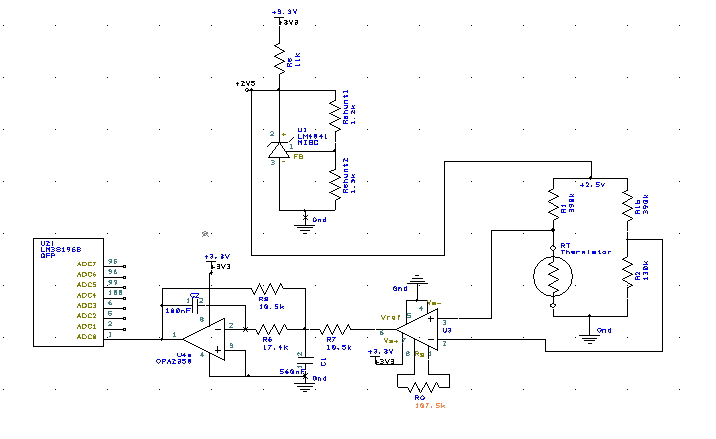
\includegraphics[width=\textwidth]{Lab9_schematic}
\vskip 0.1in
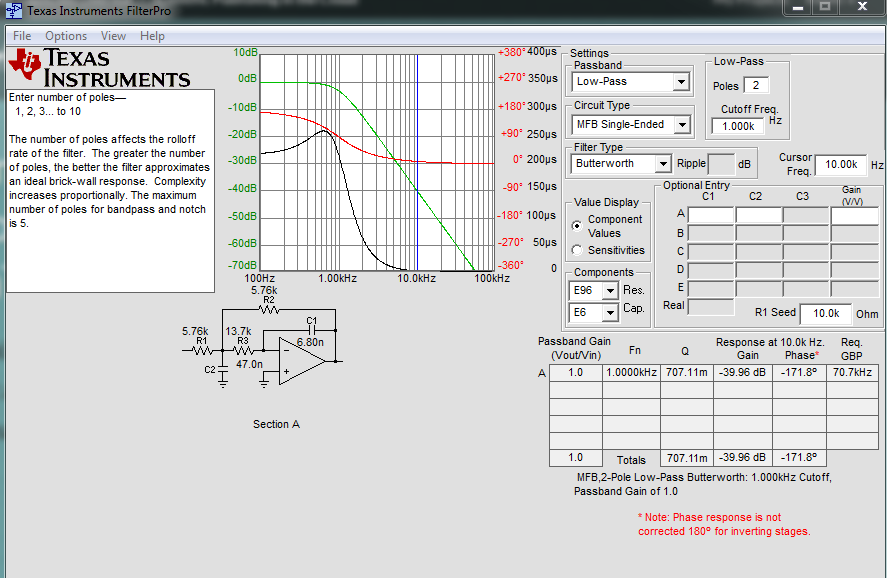
\includegraphics[width=\textwidth]{butterworthFilter}
\subsection{Measurement Data}
\subsubsection{Waveforms}
\centerline{\emph{Sampling 10 times per period (Valvano Postulate)}}
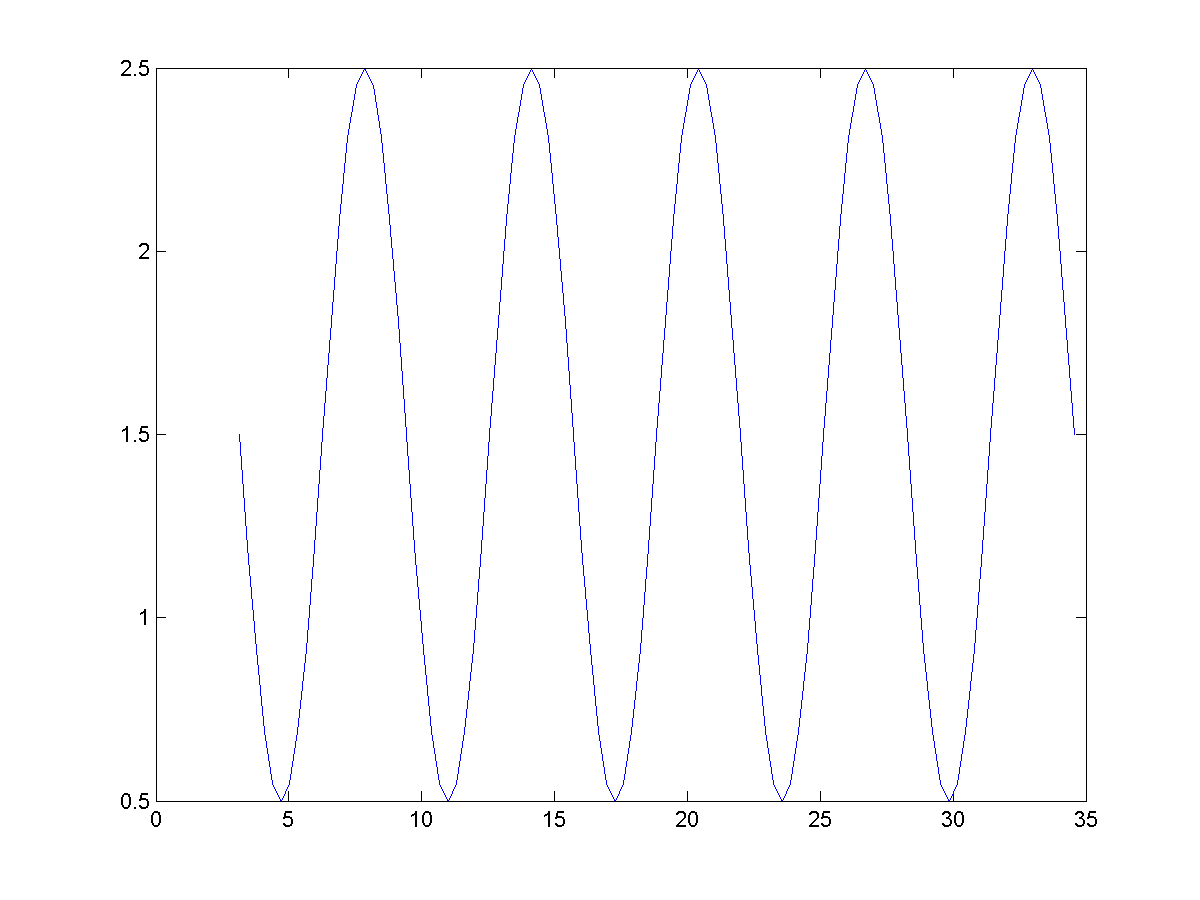
\includegraphics[height=2.5in, width=\textwidth]{valvano_postulate}
\vskip 0.1in
\centerline{\emph{Sampling twice per period (Nyquist Theorem)}}
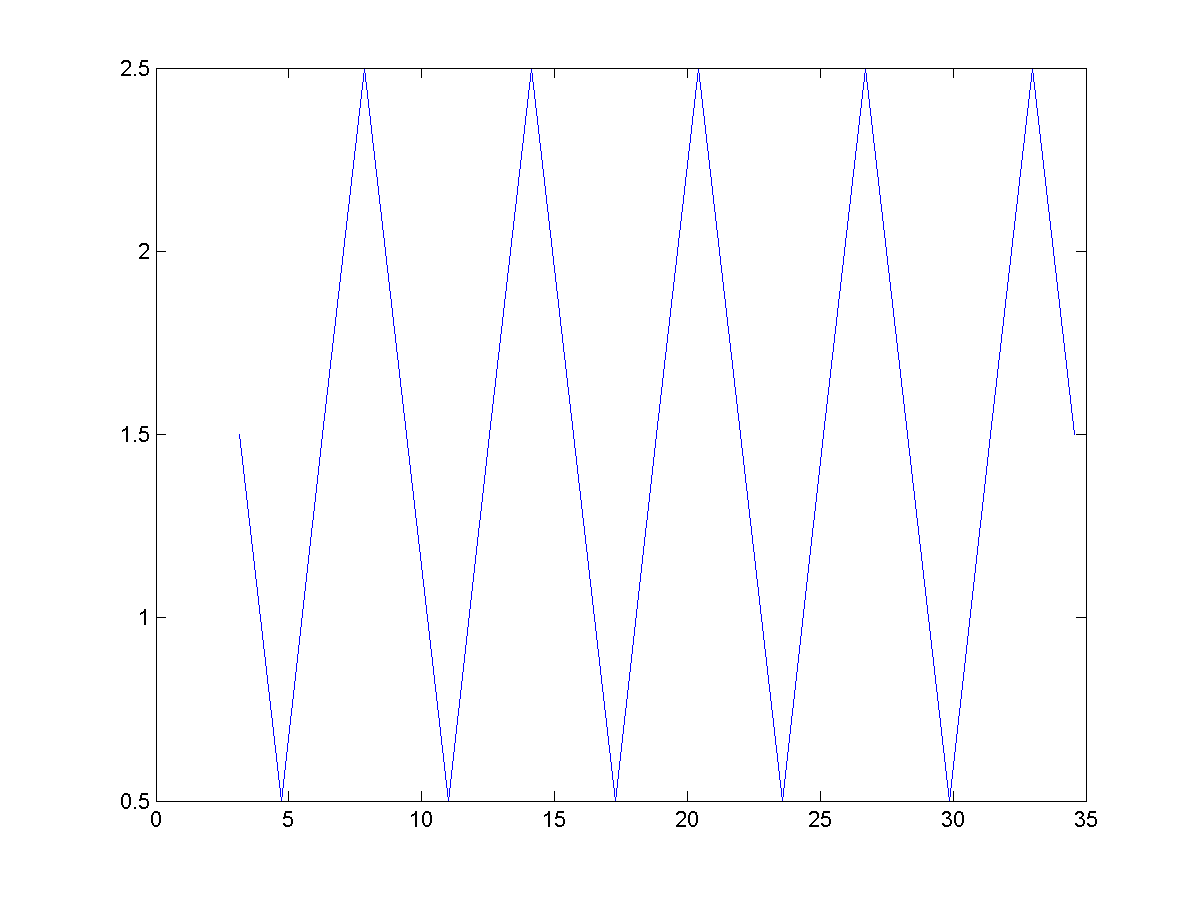
\includegraphics[height=2.5in, width=\textwidth]{nyquist_only}
\vskip 0.1in
\centerline{\emph{Sampling once every other period (aliasing). Graph overlay}}
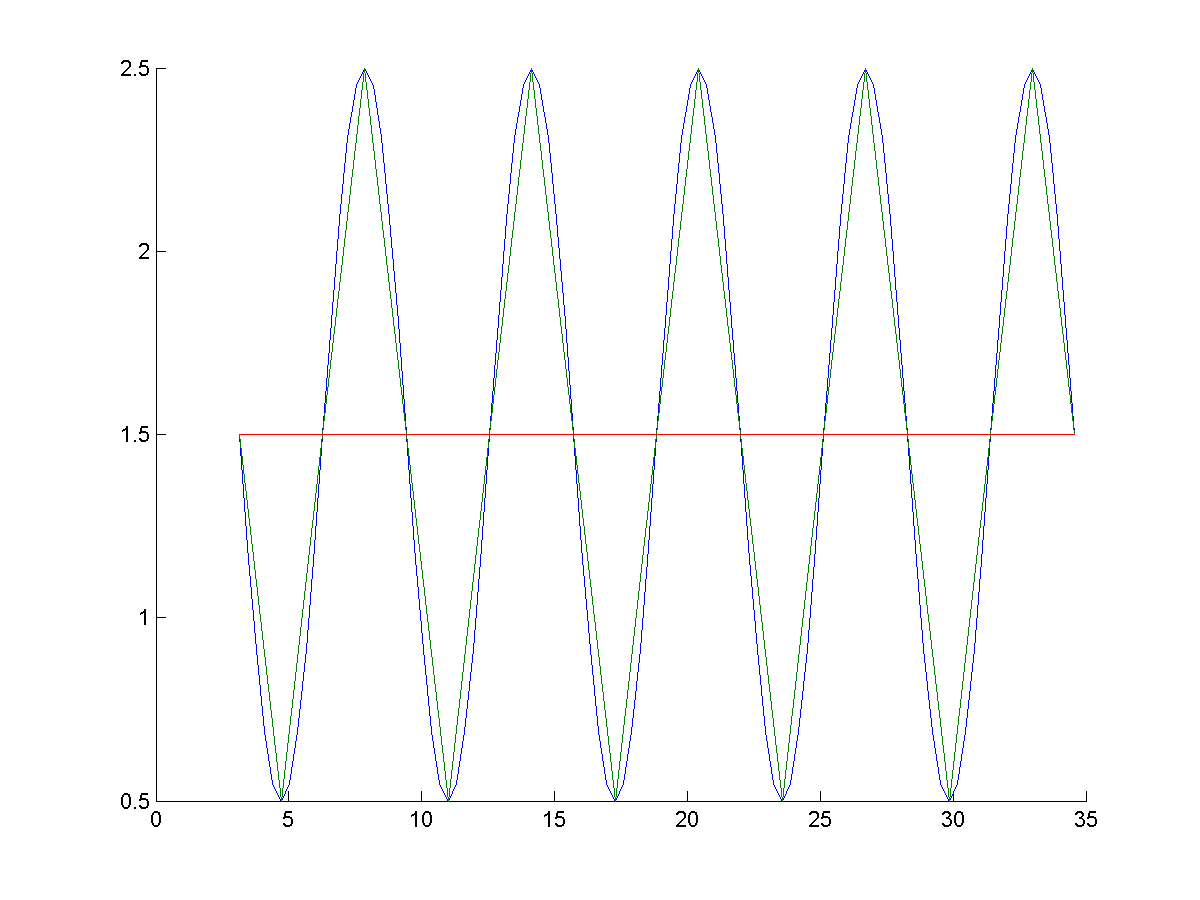
\includegraphics[height=2.5in, width=\textwidth]{nyquist_sampling_plot}
\vskip 0.1in


\subsubsection{Static Values}
\begin{enumerate}
	\item Resistor: 9.5k$\Omega$ -> 807(ADC)
    \item Resistor: 8k$\Omega$ -> 520(ADC)
    \item Resistor: 7k$\Omega$ -> 310(ADC)
    \item Resistor: 6k$\Omega$ -> 112(ADC)   
\end{enumerate}
\subsubsection{Dynamic Circuit performance}

\subsection{Analysis and Discussion}

\begin{pset}
  \problem{1:}
  \textbf{What is the Nyquist theorem and how does it apply to this lab?}\\
  	\emph{The Nyquist Theorem states that the minimum sampling frequency of an analog signal in the time domain is twice the frequency of the signal being sampled. In this lab, we needed to sample a signal coming from our thermosister.}
    
  \problem{2:}
  \textbf{Explain the difference between resolution and accuracy.}\\
  \emph{Resolution is the number of discreet values that can be measured, while accuracy measures how close those values are to the real world data. For example, how many degrees was our temperature system from a room measuring 22 degrees Celsuis. Resolution and accuracy are dependent on the same base parameters, but accuracy also depends on the reliability of the hardware, stability of the environment, and quality of the calibration.}
  
  \problem{3:}
  \textbf{Derive an equation to relate reproducibility and precision of the thermometer.}\\
  \emph{reproducibility = 2$^{10}$(precision) * 10$^{-4}$}
  
  \problem{4:}
  \textbf{What is the purpose of the LPF?}\\
  \emph{The Butterworth Low-Pass Filter was used to allow low frequency signals to be measured by the ADC. This reduced jitter and noise from the system introduced by unstable high-frequency resistances from the thermosister.}
  
  \problem{5:}
  \textbf{If the R versus T curve of the thermistor is so nonlinear, why does the voltage versus temperature curve look so linear?}\\
  \emph{If we take the voltage versus temperature curve to be in a logrithmic scale, it would appear linear.}\\
  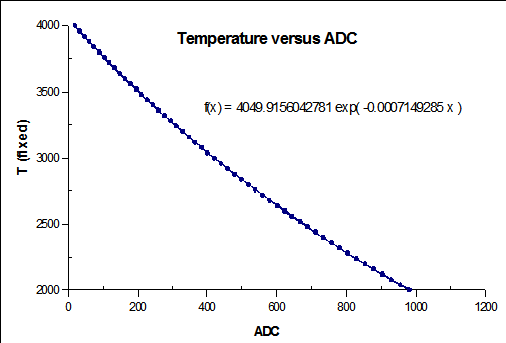
\includegraphics[height = 4in, width=\textwidth]{T_ADC}
  
  \problem{6:}
  \textbf{There are four methods (a,b,c,d) listed in the 4) Software Conversion section of methods and constraints. For one of the methods you did not implement, give reasons why your method is better, and give reasons why this alternative method would have been better. }\\
	\emph{The method that we implemented was to use a timer internally connected to the ADC to create a hardware trigger. This method has no sampling jitter since the ISR simply read s the data, acknowleges the interrput, and passes the data to the foreground using a mailbox. The other method uses a SysTick periodic interrput at the desired sampling rate and does the ADC conversions in the ISR to place them in the foreground through a mailbox. This method is simpler to implement and conceptualize.}
\end{pset}


\end{document}